\documentclass[10pt,a4paper,final]{article} %draft

\usepackage[english, russian]{babel}

\usepackage[final]{pdfpages}

\usepackage{textcomp,enumitem}

\usepackage{amsmath,amsthm,amssymb}

\usepackage{listings}
\usepackage{xcolor}
\usepackage{caption}

\definecolor{codegray}{rgb}{0.95,0.95,0.95}
\definecolor{codepurple}{rgb}{0.58,0,0.82}
\definecolor{codegreen}{rgb}{0,0.5,0} % зеленый цвет
\definecolor{codeblue}{rgb}{0,0,0.5} % синий цвет
\definecolor{codestring}{rgb}{0.64,0.08,0.08} % цвет строк


\lstset{
	language=C++,
	extendedchars=true,
	literate=
	{а}{{\selectfont\char224}}1
	{б}{{\selectfont\char225}}1
	{в}{{\selectfont\char226}}1
	{г}{{\selectfont\char227}}1
	{д}{{\selectfont\char228}}1
	{е}{{\selectfont\char229}}1
	{ж}{{\selectfont\char230}}1
	{з}{{\selectfont\char231}}1
	{и}{{\selectfont\char232}}1
	{й}{{\selectfont\char233}}1
	{к}{{\selectfont\char234}}1
	{л}{{\selectfont\char235}}1
	{м}{{\selectfont\char236}}1
	{н}{{\selectfont\char237}}1
	{о}{{\selectfont\char238}}1
	{п}{{\selectfont\char239}}1
	{р}{{\selectfont\char240}}1
	{с}{{\selectfont\char241}}1
	{т}{{\selectfont\char242}}1
	{у}{{\selectfont\char243}}1
	{ф}{{\selectfont\char244}}1
	{х}{{\selectfont\char245}}1
	{ц}{{\selectfont\char246}}1
	{ч}{{\selectfont\char247}}1
	{ш}{{\selectfont\char248}}1
	{щ}{{\selectfont\char249}}1
	{ъ}{{\selectfont\char250}}1
	{ы}{{\selectfont\char251}}1
	{ь}{{\selectfont\char252}}1
	{э}{{\selectfont\char253}}1
	{ю}{{\selectfont\char254}}1
	{я}{{\selectfont\char255}}1
	{А}{{\selectfont\char192}}1
	{Б}{{\selectfont\char193}}1
	{В}{{\selectfont\char194}}1
	{Г}{{\selectfont\char195}}1
	{Д}{{\selectfont\char196}}1
	{Е}{{\selectfont\char197}}1
	{Ж}{{\selectfont\char198}}1
	{З}{{\selectfont\char199}}1
	{И}{{\selectfont\char200}}1
	{Й}{{\selectfont\char201}}1
	{К}{{\selectfont\char202}}1
	{Л}{{\selectfont\char203}}1
	{М}{{\selectfont\char204}}1
	{Н}{{\selectfont\char205}}1
	{О}{{\selectfont\char206}}1
	{П}{{\selectfont\char207}}1
	{Р}{{\selectfont\char208}}1
	{С}{{\selectfont\char209}}1
	{Т}{{\selectfont\char210}}1
	{У}{{\selectfont\char211}}1
	{Ф}{{\selectfont\char212}}1
	{Х}{{\selectfont\char213}}1
	{Ц}{{\selectfont\char214}}1
	{Ч}{{\selectfont\char215}}1
	{Ш}{{\selectfont\char216}}1
	{Щ}{{\selectfont\char217}}1
	{Ъ}{{\selectfont\char218}}1
	{Ы}{{\selectfont\char219}}1
	{Ь}{{\selectfont\char220}}1
	{Э}{{\selectfont\char221}}1
	{Ю}{{\selectfont\char222}}1
	{Я}{{\selectfont\char223}}1,
	%	{|}{{\textbar}}1,
	%	{||}{{\textbar\textbar}}1
	%	{\&}{{\string&}}1
	%	{==}{{\string==}}1
	%	{\string\\}{{\string\\}}1,
	numbers=left,
	stepnumber=1,
	firstnumber=1,
	numberstyle=\tiny,
	basicstyle=\ttfamily\footnotesize,
	breakatwhitespace=false,
	breaklines=true,
	captionpos=b,
	keepspaces=true,
	showspaces=false,
	showstringspaces=false,
	showtabs=false,
	tabsize=2,
	frame=single,
	keywordstyle=\color{codeblue}, % ключевые слова
	commentstyle=\color{codegreen}, % комментарии
	stringstyle=\color{codestring}, % строки
	%identifierstyle=\color{green}, % стиль для переменных
	backgroundcolor=\color{codegray},
}
%\usepackage{fancyvrb}

%\usepackage{fancyhdr}

%\usepackage{upgreek}

%\usepackage{tipa}

%\usepackage{tikz}

%\usepackage{graphicx}

%\usepackage{pgfplots}

\usepackage{indentfirst}

%\usepackage{gensymb}

%\usepackage{amssymb}

%\usepackage{pdfpages}

\usepackage[unicode, pdftex, colorlinks, urlcolor=blue]{hyperref}

%\usepackage[T2A]{fontenc}

\usepackage[utf8]{inputenc}

%\usepackage[left=2cm,right=2cm,top=2cm,bottom=2cm,bindingo ffset=0cm]{geometry}

%\usepackage{graphics}

\linespread{1.5}

\pagestyle{plain}

%\usepackage{listings} 
%\usepackage{moreverb} 

%\setlist[enumerate,itemize]{leftmargin=1.2cm} %отступ в перечислениях

\hypersetup{
	colorlinks=true,
	linkcolor=black,
	%allcolors=[RGB]{0 0 0}}
}
%\lstloadlanguages{ [LaTeX] TeX}

\lstloadlanguages{ [LaTeX] TeX}



\textheight=24cm 
\textwidth=16cm
\oddsidemargin=0pt 
\topmargin=-1.5cm
\parindent=24pt 
\parskip=0pt 
\tolerance=2000 
\flushbottom 

%\usepackage[font=scriptsize]{caption}
\usepackage[labelsep=period]{caption}


\begin{document}
	\thispagestyle{empty}
	
	\begin{center}
		{\Large МИНОБРНАУКИ РОССИИ}\\
		~\\
		{\large ФЕДЕРАЛЬНОЕ ГОСУДАРСТВЕННОЕ БЮДЖЕТНОЕ ОБРАЗОВАТЕЛЬНОЕ УЧРЕЖДЕНИЕ ВЫСШЕГО ПРОФЕССИОНАЛЬНОГО ОБРАЗОВАНИЯ}\\
		~\\
		{\Large \bf <<САНКТ-ПЕТЕРБУРГСКИЙ ПОЛИТЕХНИЧЕСКИЙ УНИВЕРСИТЕТ ПЕТРА ВЕЛИКОГО>>}\\
		~\\
		{\large Институт компьютерных наук и кибербезопасности}\\
		{\large Высшая школа технологий искусственного интеллекта}\\
		{\large Направление 02.03.01 Математика и компьютерные науки}\\
		~\\
		~\\
		~\\
		~\\
		{\Large \bf Отчет по курсовой работе}\\
			{\Large по дисциплине <<Дискретная математика>> }\\
				{\Large Вариант 20.}\\
		~\\
		~\\
		{\Large  Калькулятор <<большой>> конечной арифметики.}\\
		%	{\Large \bf }\\
		~\\
		~\\
		~\\
		~\\
		~\\
		~\\
		~\\
		{\large Обучающийся: \underline{\hspace{3.5cm}} \qquad\qquad Гладков И.А.}\\
		~\\
		{\large Руководитель: \underline{\hspace{3.5cm}} \hspace{14mm} Востров А.В.}\\
		~\\
		~\\
	\end{center}
	\begin{flushright}
		
		«\underline{\hspace{1cm}}»\underline{\hspace{3cm}}20\underline{\hspace{0.7cm}}г.
	\end{flushright}
	~\\
	\begin{center}
		{\large Санкт-Петербург, 2024}
	\end{center}
	\newpage
	

	\tableofcontents
	
	\newpage
	\section* {Введение}
	\addcontentsline{toc}{section}{Введение}

	Целью данной курсовой работы является разработка и реализация калькулятора <<большой>> конечной арифметики $<Z_8;+,*>$, то есть программы, которая может выполнять арифметические операции $(+,-,*,\div)$ над числами в конечном кольце $<Z_8;+,*>$. Для этого используется основание <<малой>> конечной арифметики, в которой сложение и умножение определены по правилу <<+1>>, а также выполняются следующие свойства:коммутативность(+, *), ассоциативность(+, *), дистрибутивность * относительно +, существование нейтральных элементов: аддитивная единица <<a>> и мультипликативная единица <<b>>. Программа также обеспечивает корректность ввода данных от пользователя и выводит результаты в удобном для чтения формате. Ниже представлено правило <<+1>> для данной курсовой работы.
	
	\begin{table}[h]
		\hspace{5em} % Уменьшаем расстояние
		\centering
		\begin{minipage}{.5\textwidth}
			\centering
			\begin{tabular}{c|c c c c c c c c}
				$+$ & a & b & c & d & e & f & g & h \\
				\hline
				b & b & f & a & g & d & h & c & e \\
			\end{tabular}
			
		\end{minipage}
		%\caption{Правило <<+1>>.}
	\end{table}
	

	
		\newpage
	\section {Математическое описание}
	В этом разделе рассмотрены понятия и алгоритмы, которые лежат в основе реализации лабораторной работы.
	
	\subsection{Алгебраические структуры}

	Всюду определённая (тотальная) функция $\phi: M^n \rightarrow M$ называется n-арной(n-местной) операцией на М. Если операция $\phi$ — бинарная $\phi: (M \times M \rightarrow M)$, то будем писать в инфиксной форме $a \phi b$ вместо $\phi(a, b)$ или $ a * b$ , где * — знак операции. Множество М вместе с набором операций $\sum = \left\{\phi_1, \dots, \phi_m\right\}, \phi_i: M^{n_i} \rightarrow M$, где $n_i$ — арность операции $\phi_i$, называется алгебраической структурой, универсальной алгеброй или просто алгеброй. При этом множество М называется основным (несущим) множеством или основой (носителем); вектор арностей $(n_1, \dots ,n_m)$ называется типом; множество операций $\sum$ называется сигнатурой. Операции $\phi_i$ конечноместны, сигнатура $\sum $ конечна. Носитель не обязательно конечен, но пе пуст.
	
	\subsubsection{Конечное коммутативное кольцо с единицей}
	
	Пусть $M$ - конечное множество, а $+$ и $*$ - две операции на $M$. Тогда $M$ называется конечным коммутативным кольцом с единицей, если выполняются следующие условия:
	
	- $x+y=y+x$ и $x * y=y * x, \forall x, y \in M$ (коммутативность).
	
	- $(x+y)+c=x+(y+c)$ и $(x * y) * c=x * (y * c) \forall x, y, c \in M$ (ассоциативность).
	
	- $x * (y+c)=a * y+x * c$ и $(y+c) * x=y * x+c * x \forall x, y, c \in M$ (дистрибутивность).
	
	- $\exists a \in M$ : $x+a=a+x=x \forall x \in M$ (нейтральный элемент относительно сложения: аддитивная единица).
	
	- $\exists b \in M : x * b=b * x=x \forall x \in M$ (нейтральный элемент относительно умножения: мультипликативная единица).
	
	- $\forall x \in M \exists -x \in M : x+(-x)=(-x)+x=0$ (противоположный элемент относительно сложения).
	
	- Если $x * y=0$, то либо $x=0$, либо $y=0$  (отсутствие нетривиальных делителей нуля).
	
	Но кольце не все элементы имеют мультипликативный обратный, поэтому это свойство отсутствует. Примерами конечных коммутативных колец с единицей являются множество целых чисел, а также «малая» и «большая» конечные арифметики.
	
	«Малая» конечная арифметика - это множество с двумя операциями, похожими на сложение и умножение. Эта алгебраическая структура обозначается как $<M ;+, *>$. На множестве M также определены операции <<вычитания>> и частично <<деления>>.
	
	В этой курсовой работе множество $M_{8}$ состоит из 8 элементов, для которых действует правило <<+1>>: $\{a, b, c, d, e, f, g, h\}$. «Малую» конечную арифметику можно расширить до «большой» конечной арифметики, используя
	множество n-значных чисел, с арифметикой над $M_{8}$. В этой курсовой работе мы работаем с 8-значными числами, поэтому <<большая>> конечная арифметика обозначается как $<M_{8}^{8} ;+, *>$. Также стоит упомянуть, что на множестве $M_{8}^{8}$ определено действие <<деление с остатком>>.
	
	\section*{1.2 Вычисления отношения строгого линейного порядка и таблиц «малой» конечной арифметики}
	
	Как упоминалось ранее, для варианта 20 этой курсовой работы было установлено следующее дополнительное правило, обозначаемое как <<+1>>:
	
	\begin{table}[h]
		\hspace{5em} % Уменьшаем расстояние
		\centering
		\begin{minipage}{.5\textwidth}
			\centering
			\begin{tabular}{c|c c c c c c c c}
				$+$ & a & b & c & d & e & f & g & h \\
				\hline
				b & b & f & a & g & d & h & c & e \\
			\end{tabular}
			
		\end{minipage}
		%\caption{Правило <<+1>>.}
	\end{table}
	
	Как можно заметить, правило <<+1>> соответствует требованию <<единственности результата>>. Имея в виду, что \( a \) является минимальным элементом, а \( a + b \) представляет <<единицу>> в <<малой>> конечной арифметике, после выполнения ряда вычислений можно определить отношение строгого линейного порядка:
	
	\begin{enumerate}
		\item $a+b=b$
		\item $b+b=f$
		\item $f+b=h$
		\item $h+b=e$
		\item $e+b=d$
		\item $d+b=g$
		\item $g+b=c$
	\end{enumerate}
	
	В процессе вычислений с 1 по 7 находится наименьший элемент, который больше текущего элемента. Полученное отношение строгого линейного порядка представлено на рисунке 1:
	
		\begin{figure}[h!]
		\centering
		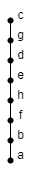
\includegraphics[width=0.08\textwidth]{2}
		\caption{Отношение строгого линейного порядка.}
	\end{figure}
	
	Для сложения <<малой>> конечной арифметики, нужно использовать полученное отношение и представить каждый элемент как сумму единиц. Тогда сложение двух элементов будет равно сумме их единиц, с учётом перехода от максимального элемента к минимальному. Например, e + h = 4 единицы + 3 единицы = 7 единиц = c. Также можно составить таблицу <<переноса по сложению>>, в которой указано, сколько раз нужно переходить от максимального элемента к минимальному при сложении. Таблицы <<сложения>> и <<переноса по сложению>> показаны на таблицах 1 и 2. Аналогично можно составить таблицу умножения <<малой>> конечной арифметики, только необходимо находить не сумму единиц, а их произведение. Например, e + h = 4 единицы * 3 единицы = 12 единиц = 8 единиц + 4 единицы, следовательно получаем 1 перенос = b и 4 единицы = e. Таблицы <<умножения>> и <<переноса по умножению>> показаны на таблицах 3 и 4.
	
	\section*{1.3 Таблицы операций малой конечной арифметики}
	
	Ниже представлены таблицы 1-4, которые отображают операции сложения и умножения с определенными нейтральными элементами для операции сложения (элемент а) и умножения (элемент b).
	\begin{table}[h!]
		\centering
		\begin{minipage}{.5\textwidth}
			\centering
			\begin{tabular}{c|cccccccc}
				
				$+$ & a & b & c & d & e & f & g & h \\
				\hline
				a & a & b & c & d & e & f & g & h \\
				b & b & f & a & g & d & h & c & e \\
				c & c & a & g & e & h & b & d & f \\
				d & d & g & e & f & b & c & h & a \\
				e & e & d & h & b & a & g & f & c \\
				f & f & h & b & c & g & e & a & d \\
				g & g & c & d & h & f & a & e & b \\
				h & h & e & f & a & c & d & b & g \\
				
			\end{tabular}
			\caption{Сложение.}
		\end{minipage}%
		\begin{minipage}{.5\textwidth}
			\centering
			\begin{tabular}{c|cccccccc}
				
				$+_s$ & a & b & c & d & e & f & g & h \\
				\hline
				a & a & a & a & a & a & a & a & a \\
				b & a & a & b & a & a & a & a & a \\
				c & a & b & b & b & b & b & b & b \\
				d & a & a & b & b & b & a & b & b \\
				e & a & a & b & b & b & a & b & a \\
				f & a & a & b & a & a & a & b & a \\
				g & a & a & b & b & b & b & b & b \\
				h & a & a & b & b & a & a & b & a \\
				
			\end{tabular}
			\caption{Перенос по сложению.}
		\end{minipage}
	\end{table}
	
	
	
	\begin{table}[h]
		\centering
		\begin{minipage}{.5\textwidth}
			\centering
			\begin{tabular}{c|cccccccc}
				
				$*$ & a & b & c & d & e & f & g & h \\
				\hline
				a & a & a & a & a & a & a & a & a \\
				b & a & b & c & d & e & f & g & h \\
				c & a & c & b & h & e & g & f & d \\
				d & a & d & h & b & e & f & g & c \\
				e & a & e & e & e & a & a & a & e \\
				f & a & f & g & f & a & e & e & g \\
				g & a & g & f & g & a & e & e & f \\
				h & a & h & d & c & e & g & f & b \\
				
			\end{tabular}
			\caption{Умножение.}
		\end{minipage}%
		\begin{minipage}{.5\textwidth}
			\centering
			\begin{tabular}{c|cccccccc}

				$*_s$ & a & b & c & d & e & f & g & h \\
				\hline
				a & a & a & a & a & a & a & a & a \\
				b & a & a & a & a & a & a & a & a \\
				c & a & a & g & e & h & b & d & f \\
				d & a & a & e & h & f & b & h & b \\
				e & a & a & h & f & f & b & h & b \\
				f & a & a & b & b & b & a & b & a \\
				g & a & a & d & h & h & b & e & f \\
				h & a & a & f & b & b & a & f & b \\
				
			\end{tabular}
			\caption{Перенос по умножению.}
		\end{minipage}
	\end{table}
	
	Примеры вычисления значений для таблиц сложения переноса по сложения(таблица 1-2):\\
		В данных расчетах перенос будет указываться в квадратных скобках и будет увеличиваться на <<b>> (мультипликативная единица) при проходжении от максимального элемента к минимальному по таблице правила <<+1>>
		\begin{enumerate}[itemsep=0pt,parsep=0pt,topsep=0pt,partopsep=0pt,label=\textbullet]
		
			\item $d+a=[a]d$, так как <<а>> - аддитивная единица
			\item $d+b=[a]g$, так как <<b>> - мультипликативная единица (правило <<+1>>)
			\item $d+c=(d+g)+b=(d+d)+b+b=(d+e)+b+b+b=(d+h)+b+b+b+b=(d+f)+b+b+b+b+b=(d+b)+b+b+b+b+b+b=
		[a](g+b)+b+b+b+b+b=[a](c+b)+b+b+b+b=[b](a+b)+b+b+b=[b](b+b)+b+b=[b](f+b)+b=h+b=e$
		\end{enumerate}
		
	Примеры вычисления значений для таблиц умножения переноса по умножения(таблица 1-2):\\
			В данных расчетах прри сложении элементов значения будут браться из таблицы слажения, переносы будут указываться в квадратных скобках и будут увеличиваться на значения из таблицы перехеодов по сложению при сложении двух элементов в примере.
	
	\begin{enumerate}[itemsep=0pt,parsep=0pt,topsep=0pt,partopsep=0pt,label=\textbullet]
	
		\item $d*b=[a]a$, так как <<а>> - аддитивная единица
		\item $d*b=[a]d$ , так как <<b>> - мультипликативная единица
		\item $d*c=d*(g+b)=
		d*(g+b)=d*(d+b+b)=d*(e+b+b+b)=d*(h+b+b+b+b)=d*(f+b+b+b+b+b)=d*(b+b+b+b+b+b+b)=(d+d)+d+d+d+d+d=
		[b](f+d)+d+d+d+d=[b](c+d)+d+d+d=[f](e+d)+d+d=[h](b+d)+d=[h]g+d=[e]h.$
		
	\end{enumerate}
	
	\newpage
	
	\section{Особенности реализации}
	\subsection{Класс Ar}
	Класс Tabl -- основной класс в курсовой работе. Опираясь на правило <<+1>> класс создает таблицы малой конечной арифметики. Затем по созданным данным расширяет малую арифметику до большой конечной, используя множество 8-разрядных чисел. Он добавляет операции вычитания и деления с отатком.  
	В классе Ar используются следующие переменные:
	\begin{enumerate}[itemsep=0pt,parsep=0pt,topsep=0pt,partopsep=0pt]
		\item vector <char> PlusOneChar -- массив хранящий внутри себя правило <<+1>>, то есть содержащий символы, которые представляют собой результат сложения каждого символа с единицей.
		\item char Graph[8] -- массив, представляющий отношение порядка между символами.
		\item regex power -- регулярное выражение для проверки вводимых чисел.
		\item string buf -- строка, в которую записывается ввод пользователя, при выборе действия в главном меню.
		\item string a -- строка отвечающая за первый число в операциях.
		\item string b -- строка отвечающая за первый число в операциях.
		\item char OperatorPlusChar[8][8] -- массив, хранящий в себе значения таблицы сложения.
		\item char OperatorPlusChar\_Shift[8][8]-- массив, хранящий в себе значения таблицы переноса по сложения.
		\item char OperatorMultChar[8][8] -- массив, хранящий в себе значения таблицы умножения.
		\item char OperatorMultChar\_Shift[8][8] -- массив, хранящий в себе значения таблицы переноса по умножению
		\item char Dictionary[8] = { 'a','b','c','d','e','f','g','h' } -- массив хранящий числа как бы в алфавитном порядке(так будут идти числа в названиях строк и столбцов всех таблиц, так удобнее для восприятия пользователем). Также в описаниях он будет называться массивом названий.
	\end{enumerate}
	
	\subsubsection{Конструктор Ar}
	Вход: создание таблицы правила <<+1>>, отношение порядка, а также таблиц сложения , переноса по сложению, умножения и переноса по умножению.
	
	Выход: сформированные отношение порядка и таблиц правила <<+1>> сложения , переноса по сложению, умножения и переноса по умножению.
	
	Вначале в массив отвечающий за правило <<+1>> добавляются элементы, порядок элементов производится в соответствии с вариантом. После формируются отношение порядка. Формируется регулярное выражение для корректности ввода числа пользователем. Затем вызываются методы формирования таблиц сложения, переноса по сложению, умножения и переноса по умножению(листинг 1).
	
	\begin{lstlisting}[caption={Конструктор Ar}]
		Ar::Ar() {
			PlusOneChar.push_back('b');
			PlusOneChar.push_back('f');
			PlusOneChar.push_back('a');
			PlusOneChar.push_back('g');
			PlusOneChar.push_back('d');
			PlusOneChar.push_back('h');
			PlusOneChar.push_back('c');
			PlusOneChar.push_back('e');

			Graph[0] = 'a';
			Graph[1] = 'b';
			Graph[2] = 'f';
			Graph[3] = 'h';
			Graph[4] = 'e';
			Graph[5] = 'd';
			Graph[6] = 'g';
			Graph[7] = 'c';
			
			power= ("^(-?[a-h]{1,8})$");
			
			CreateOperatorPlus();
			CreateOperator_Shift(OperatorPlusChar_Shift,0);
			CreateOperatorMult();
			CreateOperator_Shift(OperatorMultChar_Shift,1);
		}
	\end{lstlisting}
	
		\subsubsection{Конструктор CreateOperatorPlus}
	Вход: создание таблицы сложения.
	
	Выход: сформированная таблица сложения.
	
	Первая строчка и первый столбец таблицы сложения -- это все цифры, которые как бы идут в алфавитном порядке, но на самом деле у них разные значения, это проще для визуального восприятия в таблице. Вторая строчка и второй столбец -- это числа из таблицы <<+1>>, повторяющие порядок, так как просто прибавляется <<b>>, то есть мультипликативная единица. Далее находятся все остальные значения таблицы при помощи метода Summ, и записываются сразу в два поля таблицы, так как она симметричная. Листинг 2.
	
	\begin{lstlisting}[caption={Конструктор CreateOperatorPlus}]
		void Ar::CreateOperatorPlus() {
			for (int i = 0; i < 8; i++) {
				OperatorPlusChar[i][0] = Dictionary[i];
				OperatorPlusChar[0][i] = Dictionary[i];
				OperatorPlusChar[i][1] = PlusOneChar[i];
				OperatorPlusChar[1][i] = PlusOneChar[i];
			}
			
			for (int i = 2; i < 8; i++) {
				for (int j = i; j < 8; j++) {
					char buf = Summ(Dictionary[i], Dictionary[j]);
					OperatorPlusChar[i][j] = buf;
					OperatorPlusChar[j][i] = buf;
					
				}
			}
		}
	\end{lstlisting}
	
	\subsubsection{Метод Summ}
	Вход: два символа из таблицы которые нужно сложить
	
	Выход: результат сложения входных символов.
	
	Значения находятся по сумме количеств мультипликативных единиц(<<b>>) в числах, а точнее считает сколько <<b>> во втором числе операции, потом к первому числу прибавляет единицу нужное количесво раз по правилу <<+1>>(листинг 3). В методе используются методы SearchIndex DictionaryToInt. Они будут описаны ниже, листинге 4-5.
	
		\begin{lstlisting}[caption={Метод Summ}]
char Ar::Summ(char a, char b) {
	int k = 0;
	char result = a;
	char buf = b;
	char check = b;
	while (check != 'b') {
		buf = Dictionary[SearchIndex(buf)];
		check = PlusOneChar[DictionaryToInt(buf)];
		k++;
	}
	while (k > 0) {
		result = PlusOneChar[DictionaryToInt(result)];
		k--;
	}
	return result;
}
	\end{lstlisting}
	
		\subsubsection{Методы SearchIndex, DictionaryToInt, SearchInGraph}
		Метод SearchIndex находит индекс в массиве, который отвечает за правило <<+1>>. Используется в методах, где необходимо начать прибавлять по одному начиная с какогото числа.
		
	Вход: число, индекс которого необходимо найти.
	
	Выход: индекс входного числа в массиве правила <<+1>>
	
		\begin{lstlisting}[caption={Метод SearchIndex}]
		int Ar::SearchIndex(char a) {
			for (int i = 0; i < 8; i++)
			if (PlusOneChar[i]== a)
			return i;
		};
	\end{lstlisting}
	
		Метод DictionaryToInt находит индекс цифры в строке или столбце названий таблиц. Используется в различных методах, где это необходимо.
		
		Вход: число, индекс которого необходимо найти.
		
		Выход: индекс входного числа в массиве названий.
		
		
	\begin{lstlisting}[caption={Метод DictionaryToInt}]
		int Ar::DictionaryToInt(char s) {
			for (int i = 0; i < 8; i++) {
				if (Dictionary[i] == s)
				return i;
			}
		}
	\end{lstlisting}
	
	Метод SearchInGraph находит индекс числа в массиве отношении порядка, можно сказать, что он находит количество единиц в цифре. Используется в различных методах, где это необходимо.

Вход: число, индекст которого необходимо найти.

Выход: индекс входного числа в массиве отношении порядка, то есть количество единиц в цифре.
	
		
			\begin{lstlisting}[caption={Метод SearchInGraph}]
					int Ar::SearchInGraph(char a) {
					for (int i = 0; i < 8; i++)
					if (a == Graph[i])
					return i;
				};
		\end{lstlisting}
		
			\subsubsection{Метод CreateOperatorMult}
				Вход: создание таблицы умножения.
			
			Выход: сформированная таблица умножения.
			
			Первая строчка и первый столбец таблицы умножения -- это аддитивные единицы, а именно цифры <<a>>. Вторая строчка и второй столбец -- это числа из таблицы значений. Далее находятся все остальные значения таблицы при помощи метода Mult, и записываются сразу в два поля таблицы, так как она симметричная. Смотрите листинг 7.
		
		
		\begin{lstlisting}[caption={Метод CreateOperatorMult}]
			void Ar::CreateOperatorMult() {
				for (int i = 0; i < 8; i++) {
					OperatorMultChar[i][0] = 'a';
					OperatorMultChar[0][i] = 'a';
					OperatorMultChar[i][1] = Dictionary[i];
					OperatorMultChar[1][i] = Dictionary[i];
				}
				for (int i = 2; i < 8; i++) {
					for (int j = i; j < 8; j++) {
						char buf = Mult(Dictionary[i], Dictionary[j]);
						OperatorMultChar[i][j] = buf;
						OperatorMultChar[j][i] = buf;
						
					}
				}
			}
		\end{lstlisting}
		
			\subsubsection{Метод Mult}
		Вход: два символа из таблицы которые нужно перемножить.
		
		Выход: результат произведения входных символов.
		
		Находится количество <<b>> во второй числе операции, затем данное количество раз будет складываться первое число с самим собой, то есть происходит умножение (листинг 8). Для реализации данных чисел используется метод SearchInPlus, описанный ниже, в листинге 10. 
		\begin{lstlisting}[caption={Метод Mult}]
	char Ar::Mult(char a, char b) {
		char result = a;
		char buf = a;
		int k = SearchInGraph(b) - 1;
		while (k > 0) {
			result = SearchInPlus(result, buf);
			k--;
		}
		return result;
	}
		\end{lstlisting}
		
		\subsubsection{Метод CreateOperator\_Shift}
			Вход: флаг, показывающий операцию: 1 - умножение, 0 - сложения. 
		
		Выход: сформированный массив переноса по умножению, либо по сложению, в зависимости от входного параметра.
		
		В методе происходит, либо умножение, либо сложение количества единиц двух цифр, в зависимости от входного параметра. Затем результат делится на 8 и результат деления находится в таблице отношения порядка, то есть результирующее количество единиц интерпретируется в цифру по таблице отношения порядка.
					
		\begin{lstlisting}[caption={Метод CreateOperator\_Shift}]
			void Ar::CreateOperator_Shift( bool flag) {
				int k;
				for (int i = 0; i < 8; i++) {
					for (int j = 0; j < 8; j++) {
						k = flag? SearchInGraph(Dictionary[i]) * SearchInGraph(Dictionary[j]) 
						: SearchInGraph(Dictionary[i]) + SearchInGraph(Dictionary[j]);
						k = k / 8;
						if (flag)
						OperatorMultChar_Shift[i][j] = Graph[k];
						else
						OperatorPlusChar_Shift[i][j] = Graph[k];
					}
				}
			}
		\end{lstlisting}
		
		\subsubsection{Методы SearchInPlus, SearchInPlus\_Shift, SearchInMult, SearchInMult\_Shift, SearchInSub}
		
		Метод SearchInPlus
		
		Вход: два символа, для которых нужно найти значени в таблице сложения.
		
		Выход: значение сложения двух символов из таблицы .
		
		В методе происходит поиск по таблице сложения, найденный результат возвращается.
		
			\begin{lstlisting}[caption={Метод SearchInPlus}]
			char Ar::SearchInPlus(char a, char b) {
				return OperatorPlusChar[DictionaryToInt(a)][DictionaryToInt(b)];
			};
		\end{lstlisting}
		
				Метод SearchInPlus\_Shift
		
		Вход: два символа, для которых нужно найти значени в таблице переноса по сложению.
		
		Выход: значение переноса при сложении двух символов из таблицы .
		
		В методе происходит поиск по таблице переноса по сложению, найденный результат возвращается.
		
		
		\begin{lstlisting}[caption={Метод SearchInPlus\_Shift}]
			char Ar::SearchInPlus_Shift(char a, char b) {
				return OperatorPlusChar_Shift[DictionaryToInt(a)][DictionaryToInt(b)];
			};
		\end{lstlisting}
		
				Метод SearchInMult
		
		Вход: два символа, для которых нужно найти значение в таблице умножения
		
		Выход: значение сложения двух символов из таблицы умножения .
		
		В методе происходит поиск по таблице умножения, найденный результат возвращается.
		
			\begin{lstlisting}[caption={Метод SearchInMult}]
			char Ar::SearchInMult(char a, char b) {	
				return OperatorMultChar[DictionaryToInt(a)][DictionaryToInt(b)];
			};
		\end{lstlisting}
		
				Метод SearchInMult\_Shift
		
		Вход: два символа, для которых нужно найти значени в таблице переноса по уменожению
		
		Выход: значение переноса приумножении двух символов из таблицы .
		В методе происходит поиск по таблице переноса по умножению, найденный результат возвращается.
		
		\begin{lstlisting}[caption={Метод SearchInMult\_Shift}]
		char Ar::SearchInMult_Shift(char a, char b) {	
			return OperatorMultChar_Shift[DictionaryToInt(a)][DictionaryToInt(b)];
		};
	\end{lstlisting}
		
		Метод SearchInSub
		
		Вход: два символа, разность которых нужно найти
		
		Выход: значение разности двух символов из таблицы сложения .
		
		В методе происходит поиск по таблице сложения, первая цифра является итогом сложения по таблице сложения, вторая будут находится в названии столбца либо строки, тогда результат будет находится в строке, либо столбце соответственно, так как таблица симметрична, относительно главной диагонали.
		
		\begin{lstlisting}[caption={Метод SearchInSub}]
		char Ar::SearchInSub(char a, char b) {	
			for (int i = 0; i < 8; i++) {
				if (OperatorPlusChar[i][DictionaryToInt(b)] == a) {
					return Dictionary[i];
				}
			}
		};
		\end{lstlisting}
		
		
		
			\subsubsection{Методы Comparasion, compare}
	
		Метод Comparasion:
		
		Вход: Два символа, которые неоходимо стравнить.
		
		Выход: вывод, первая меньше второй или нет.
		
		Метод сравнивает количество единиц в первой цифре, со второй. Если в первой меньше, то возвращается true, иначе false.
		\begin{lstlisting}[caption={Метод Comparasion}]
			bool Ar::Comparasion(char a, char b) {
				for (int i = 0; i < 8; i++) {
					for (int j = 0; j < 8; j++) {
						if (Graph[i] == a && Graph[j] == b)
						if (i < j)
						return true;
						else
						return false;
					}
				}
			}
		\end{lstlisting}
		
				Метод compare:
					
					Вход: Два числа, которые необходимо сравнить.
				
				Выход: вывод, больше, меньше, или равно.
				
				Метод сравнивает два числа начиная со старшего разряда. Если они разных разрядов, то меньшеразрядное число заполняется незначащими нулями. Далее происходит по разрядная проверка. Если разряд первого чмсла меньше второго, то выводится <<-1>> (первое число меньше второго) если больше, то <<1>>(второе число больше первого), иначе по окончании цикла выводтся <<0>>, это означает, что они равны. 
		
		\begin{lstlisting}[caption={Метод compare}]
			flag = compare(a, b);
			if ((minuses_a + minuses_b) == 1 && fl == 1
			|| (minuses_a + minuses_b) != 1 && fl == 0) {
				answer = ToSub(a, b);
				if (answer.size() > 8)
				answer = "overflow";
				if (answer != "overflow" &&
				((minuses_b == 1 && flag == -1 && fl == 1) ||
				(minuses_a == 1 && flag == 1 && fl == 1) ||
				((minuses_a + minuses_b) == 0 && flag == -1 && fl == 0) ||
				((minuses_a + minuses_b) == 2 && flag == 1 && fl == 0))) {
					answer = '-' + answer;
				}
			}
		\end{lstlisting}
		
			\subsubsection{Метод ToSumm}
			Вход: два числа, которые необходимо сложить.
			
			Выход Результат сложения двух чиселю.
			
			Метод реализует сложение в столбик, то есть сложение происходит поразрядно.Начинается все с младшего разряда. Если происходит переход при сложении, то он прибавляется к следующему разряду, и так пока не закончатся разряды.
		
		\begin{lstlisting}[caption={Метод ToSumm}]
			string Ar::ToSumm(string a, string b) {
				char shift1 = 'a';
				char shift2 = 'a';
				char shift3 = 'a';
				char solution;
				string answer = "";
				while (a.size() != b.size()) {
					a.size() < b.size() ? a = 'a' + a : b = 'a' + b;
				}
				for (int i = a.size() - 1; i >= 0; i--) {
					solution = SearchInPlus(a[i], b[i]);
					shift2 = SearchInPlus_Shift(a[i], b[i]);
					shift3 = SearchInPlus_Shift(solution, shift1);
					solution = SearchInPlus(solution, shift1);
					shift1 = SearchInPlus(shift2, shift3);
					answer = solution + answer;
					shift3 = 'a';
					shift2 = 'a';
					if (i == 0 && shift1 != 'a')
					answer = shift1 + answer;
				}
				while (answer.size() > 1 && answer[0] == 'a')
				answer.erase(0, 1);
				
				return answer;
			}
		\end{lstlisting}
		
		
			\subsubsection{Метод ToSub}
			Вход: два числа, с которыми необходимо выполить разность.

	Выход: Результат вычитания двух чисел.
	
	Метод реализует вычитание в столбик, то есть происходит поразрядно. Все начинается с младшего разряда. Если символ в первом числе меньше символа во втором, происходит уменьшение, цифра разряда старше на <<b>>, и в данном разряде происходит вычитание из наибольшого символа (той, которая содержит 7 единиц, то есть <<c>>), затем прибавляется <<b>> и после прибавляется изначальная символ, иначе с помощью метода SearchInSub нахоbдтся разность символов.Листинг 18. 
	
		\begin{lstlisting}[caption={Метод ToSub}]
			string Ar::ToSub(string a, string b) {
				int flag;
				char solution;
				string answer = "";
				flag = compare(a, b);
				if (flag == 0) {
					answer = 'a';
				}
				else {
					if (flag == -1) {
						a.swap(b);
					}
					for (int i = a.size() - 1; i >= 0; i--) {
						if (i > 0) {
							if (Comparasion(a[i], b[i])) {
								int j = i - 1;
								while (j >= 0){
									if (a[j] != 'a') {
										a[j] = SearchInSub(a[j], 'b');
										break;
									}
									else
									a[j] = SearchInSub(a[j], 'b');
									j--;
								}
								solution = SearchInSub('c', b[i]);
								solution = SearchInPlus('b', solution);
								solution = SearchInPlus(a[i], solution);
							}
							else {
								solution = SearchInSub(a[i], b[i]);
							}
							answer = solution + answer;
						}
						else {
							solution = SearchInSub(a[i], b[i]);
							answer = solution == 'a' ? answer : solution + answer;
						}
					}
				}
				while (answer.size() > 1 && answer[0] == 'a')
				answer.erase(0, 1);
				
				return answer;
			}
		\end{lstlisting}
		
		\subsubsection{Метод ToSumm\_or\_ToSub}
		
		Вход: два числа, которые ввел пользователь, либо в калькуляторе сложения, либо вычитания, а также флаг операции.
		
		Выход:конечный результат операции над данными числами.
		
		Данный метод, определяет, когда ему совершить операцию сложения, а когда вычитания, так как все зависит от входных данных, а именно у какого числа есть минус и входной флаг. Например, если флаг -- 0 (т.е. вычитание) и на вход подается первое число положительное, а второе отрицательное, то из-за правила -- минус на минус дает плюс-- стоит выполнить сложение. Или, если в сложении, одно из чисел отрицательное, то стоит выполнить вычитание. При определенных условиях вызываются методы сложение или вычитания (ToSumm, ToSub). Смотрите листинг 19.
		
		\begin{lstlisting}[caption={Метод ToSumm\_or\_ToSub}]
			string Ar::ToSumm_or_ToSub(string a, string b, bool fl) {
				string answer = "";
				int minuses_a = 0;
				int minuses_b = 0;
				int flag;
				if (a[0] == '-') {
					minuses_a++;
					a.erase(0, 1);
				}
				if (b[0] == '-') {
					minuses_b++;
					b.erase(0, 1);
				}
				while (a.size() != b.size()) {
					a.size() < b.size() ? a = 'a' + a : b = 'a' + b;
				}
				
				flag = compare(a, b);
				if ((minuses_a + minuses_b) == 1 && fl == 1
				|| (minuses_a + minuses_b) != 1 && fl == 0) {
					answer = ToSub(a, b);
					if (answer.size() > 8)
					answer = "overflow";
					if (answer != "overflow" &&
					((minuses_b == 1 && flag == -1 && fl == 1) ||
					(minuses_a == 1 && flag == 1 && fl == 1) ||
					((minuses_a + minuses_b) == 0 && flag == -1 && fl == 0) ||
					((minuses_a + minuses_b) == 2 && flag == 1 && fl == 0))) {
						answer = '-' + answer;
					}
				}
				else {
					answer = ToSumm(a, b);
					if (answer.size() > 8)
					answer = "overflow";
					if (answer != "overflow" &&
					((minuses_a == 1 && flag == 1 && fl ==0) ||
					(minuses_a == 1 && flag == -1 && fl == 0) ||
					((minuses_a + minuses_b) == 2 && flag == -1 && fl == 1) ||
					((minuses_a + minuses_b) == 2 && flag == 1 && fl == 1)))
					answer = '-' + answer;
				}
				return answer;
			}
		\end{lstlisting}
		
		
			\subsubsection{Метод ToMult\_Base}
			
			Вход: два числа, которые необходимо перемножить.
			
			Выход Результат произведения двух чисел.
			
			В данном методе прописанна оснавноая логика произведения чисел. Умножение производится в столбик: один разряд второго числа,начиная с младшего, перемножается с каждым разрядом первого числа, при этом если происходит перенос по таблице переносов по умножению, то он складывеется в более старший разряд. произведение символов находится по таблице умножения. Затем происходит возвращение результата(листинг 20).
			
		
		\begin{lstlisting}[caption={Метод ToMult\_Base}]
			
			string Ar::ToMult_Base(string a, string b) {
				string answer = "a";
				string answer_buf = "";
				char shift1 = 'a';
				char shift2 = 'a';
				char shift3 = 'a';
				char solution;
				int flag;
				
				
				int k = 0;
				for (int i = b.size() - 1; i >= 0; i--) {
					for (int j = a.size() - 1; j >= 0; j--) {
						solution = SearchInMult(a[j], b[i]);
						shift2 = SearchInMult_Shift(a[j], b[i]);
						shift3 = SearchInPlus_Shift(solution, shift1);
						solution = SearchInPlus(solution, shift1);
						shift1 = SearchInPlus(shift2, shift3);
						answer_buf = solution + answer_buf;
						shift3 = 'a';
						shift2 = 'a';
						if (j == 0 && shift1 != 'a')
						answer_buf = shift1 + answer_buf;
					}
					
					shift1 = 'a';
					int s = k;
					while (s > 0) {
						answer_buf += 'a';
						s--;
					}
					k++;
					answer = ToSumm(answer, answer_buf);
					answer_buf = "";
				}
		\end{lstlisting}
		
		
				\subsubsection{Метод ToMult}
				Вход: два числа,введенные пользователем, которые необходимо перемножить.
				
				Выход Конечный результат произведения двух чисел.
				
				Данный метод оценивает входные данные, вызывает метод ToMult\_Base, для перемножения чисел без минусов, затем на основании собранных данных, либо оставляет ответ без минусов, либо добавляет минуст в ответ(листинг 21).
		
		\begin{lstlisting}[caption={Метод ToMult}]
			string Ar::ToMult(string a, string b) {
				string answer = "a";
				int minuses_a = 0;
				int minuses_b = 0;
				if (a[0] == '-') {
					minuses_a++;
					a.erase(0, 1);
				}
				if (b[0] == '-') {
					minuses_b++;
					b.erase(0, 1);
				}
				while (a.size() != b.size()) {
					a.size() < b.size() ? a = 'a' + a : b = 'a' + b;
				}
				
				answer = ToMult_Base(a, b);
				
				while (answer.size() > 1 && answer[0] == 'a')
				answer.erase(0, 1);
				
				if (answer.size() > 8)
				answer = "overflow";
				
				if (answer[0] != 'a' && answer != "overflow" && (minuses_a + minuses_b) == 1)
				answer = '-' + answer;
				return answer;
		\end{lstlisting}
		
		
		
		\subsubsection{Метод ToDiv}
		
		Вход: два числа,введенные пользователем, которые необходимо резделить. 
		
		Выход: Конечный результат деления двух чисел.
		
		Данный метод вначале проверяет, не подается ли на вход нулевое значение (аддитивная единица), если да, то обрабатываются случаи: если делимое -- нулевое (аддитивная единица), то в ответе получаем нулевое значение(аддитивная единица), если делитель нулевой (аддитивная единица), то ответа не существет, если и делимое, и делитель -- аддитивные единицы, то ответ -- весь возможный промежуток. При четвертом случае, происходит деление модулей чисел, а именно частное увеличивается пока произведение частного на делитель, меньше или равно делимому. Когда нахоится максимальное возможное частное подходящее под условие, то после находится остаток -- разность делимого с произведением частного на делителя. Также если делимое и делитель положительные, то часное тоже положительно. Если делимое положительное и делитель отрицательное, то находится частное по модулям делителя и делимого,  после к частному прибавляется минус. Если делимое отрицательное, делитель положительный, то также находится частное их модулей, затем к частному прибавляется минус и отнимается мультипликативная единица. Если оба отрицательные, то находится частное модулей, прибавляется мультипликативная единица. Частное всегда положительное и находится по формуле: разность делимого с произведением частного на делителя. Операция деления описана в листинге 22.
		
		\begin{lstlisting}[caption={Метод ToDiv}]
			vector <string> Ar::ToDiv(string a, string b, vector<string> result) {
				//string buf = a;
				string answer = "a";// делитель
				string answer_buf = "a";//частное
				int minuses_a = 0;
				int minuses_b = 0;
				char shift1 = 'a';
				char shift2 = 'a';
				char shift3 = 'a';
				char solution;
				int flag;
				
				if (a[0] == '-') {
					minuses_a++;
					a.erase(0, 1);
				}
				if (b[0] == '-') {
					minuses_b++;
					b.erase(0, 1);
				}
				
				if (compare(a, "a") == 0 && compare(b, "a") == 0) { //две переменные равны "a" -> запысываем в вектор "1"
					result.push_back(answer);
					result.push_back(answer_buf);
					result.push_back("1");
				}
				else if (compare(a, "a") != 0 && compare(b, "a") == 0) {//только делитель равен "а" -> записываем "2"
					result.push_back(answer);
					result.push_back(answer_buf);
					result.push_back("2");
				}
				else if (compare(a, "a") == 0 && compare(b, "a") != 0) {//только делимое равено "а" -> записываем "0",
					//то есть получаем какоето число, а именно "a"
					result.push_back(answer);
					result.push_back(answer_buf);
					result.push_back("0");
				}
				else {
					
					while (a.size() != b.size()) {
						a.size() < b.size() ? a = 'a' + a : b = 'a' + b;
					}
					
					while (true) {
						if (compare(ToMult_Base(b, ToSumm(answer, "b")), a) != 1) {
							if (compare(ToMult_Base(b, ToSumm(answer, "ba")), a) != 1) {
								if (compare(ToMult_Base(b, ToSumm(answer, "baa")), a) != 1) {
									if (compare(ToMult_Base(b, ToSumm(answer, "baaa")), a) != 1) {
										if (compare(ToMult_Base(b, ToSumm(answer, "baaaa")), a) != 1) {
											if (compare(ToMult_Base(b, ToSumm(answer, "baaaaa")), a) != 1) {
												if (compare(ToMult_Base(b, ToSumm(answer, "baaaaaa")), a) != 1) {
													if (compare(ToMult_Base(b, ToSumm(answer, "baaaaaaa")), a) != 1) {
														answer = ToSumm(answer, "baaaaaaa");
													}
													else
													answer = ToSumm(answer, "baaaaaa");
												}
												else
												answer = ToSumm(answer, "baaaaa");
											}
											else
											answer = ToSumm(answer, "baaaa");
										}
										else
										answer = ToSumm(answer, "baaa");
									}
									else
									
									answer = ToSumm(answer, "baa");
								}
								else
								answer = ToSumm(answer, "ba");
							}
							else
							answer = ToSumm(answer, "b");
						}
						else
						break;
					}
					while (a.size() > 1 && a[0] == 'a')
					a.erase(0, 1);
					
					a = minuses_a == 1 ? '-' + a : a;
					
					while (b.size() > 1 && b[0] == 'a')
					b.erase(0, 1);
					
					b = minuses_b == 1 ? '-' + b : b;
					
					if (minuses_a == 0 && minuses_b == 1) {
						answer = '-' + answer;
						//answer_buf = ToSub(a, ToMult(b, answer));
					}
					else if (minuses_a == 1 && minuses_b == 0) {
						answer = '-' + answer;
						string m =  ToMult(b, answer);
						if (compare(ToMult(b, answer), a) != 0)
						answer = ToSumm_or_ToSub(answer, "b", 0); //вычитаем один
						//answer_buf = ToSub(a, ToMult(b, answer));
					}
					else if (minuses_a + minuses_b == 2) {
						if (compare(ToMult(b, answer), a) != 0)
						answer = ToSumm_or_ToSub(answer, "b", 1);// прибавляем 1
					}
					
					answer_buf = ToSumm_or_ToSub(a, ToMult(b, answer), 0);
					
					result.push_back(answer);
					result.push_back(answer_buf);
					result.push_back("0");
				}
				return result;
				
			}
		\end{lstlisting}
		
		
		\subsubsection{Метод Menu}
		
		\par Вход: ожидание вывести возможные действия работы программы пользователю.
		\par Выход: выводится меню действий на консоль, позьзователь выбирает нужное для него действие.
		\par В методе  Menu происходит вывод на экран всех возможных действий. Пользователь выбирает  нужное ему действие, при этом вызывается метод для проверки пользовательсктго ввода, дальше вызывается метот соответствующий выбору пользователя.
		\begin{lstlisting}[caption={Метод Menu}]
void Ar::Menu() {
	cout << "\n\tДобро пожаловать в калькулятор \"большой\" конечной арифметики\n";
	while (true) {
		bool out = 0;
		printf("\n\nВот что вы можете сделать:");
		printf("\n Вывести ... ");
		printf("\n [1] Правило \"+1\"");
		printf("\n [2] Таблицу сложения \"+\"");
		printf("\n [3] Таблицу умножения \"*\"");
		printf("\n [4] Отношение порядка");
		printf("\n Перейти в... ");
		printf("\n [5] Калькулятор сложения\"+\"");
		printf("\n [6] Калькулятор вычитания\"-\"");
		printf("\n [7] Калькулятор умножения\"*\"");
		printf("\n [8] Калькулятор деления\"/\"");
		printf("\n Выйти из... ");
		printf("\n [0] Программы\n\n");
		
		while (true) {
			cin >> buf;
			try {
				if (stoi(buf) >= 0 && stoi(buf) <= 8) {
					break;
				}
				else {
					std::cout << "Ошибка ввода! Ведите число от 0 до 8\n";
				}
			}
			catch (const std::invalid_argument& e) {
				std::cout << "Ошибка ввода! Неверный формат числа\n";
			}
			
		}
		int n = stoi(buf);
		
		switch (n) {
			case 0:
			out = 1;
			break;
			
			case 1:
			PrintPlusOneChar();
			break;
			
			case 2:
			PrintOperator(OperatorPlusChar);
			PrintOperator(OperatorPlusChar_Shift);
			break;
			
			case 3:
			PrintOperator(OperatorMultChar);
			PrintOperator(OperatorMultChar_Shift);
			break;
			case 4:
			PringGraph();
			break;
			
			case 5:
			SummCalculator();
			break;
			
			case 6:
			SubCalculator();
			break;
			
			case 7:
			MultCalculator();
			break;
			
			case 8:
			DivCalculator();
			break;
			
			
			
		}
		if (out)
		break;
		system("pause");
	}
}
		\end{lstlisting}
		
		
		\subsubsection{Метод DivCalculator}
		
		Вход: запрашивается у пользователя два числа для операции деления. 
		
		Выход: результат операции деления на экран с введенными числами.
		
		Метод вызывает функцию запроса числа от пользователя два раза, после вызывает функцию деления для данных чисел. Потом вывод результата на экран.  
		
		\begin{lstlisting}[caption={Метод DivCalculator}]
			void Ar::DivCalculator() {
				vector<string> answer;
				printf("\n --------------------------------------");
				printf("\n Вы перешли в калькулятор Деления.");
				printf("\n Для выхода в главное меню введите [0].\n\n");
				while (true) {
					printf("Что вы хотите поделить?\n");
					a = Check();
					if (a == "0")
					break;
					printf(" \"/\"\n");
					b = Check();
					if (b == "0")
					break;
					answer=ToDiv(a, b, answer);
					if (answer[2] == "0") {
						if (b[0] == '-')
						std::cout << "\nОтвет: " << a << " / (" << b << ") = " << answer[0] << "\n";
						else
						std::cout << "\nОтвет: " << a << " / " << b << " = " << answer[0] << "\n";
						std::cout << "       остаток = " << answer[1] << "\n\n";
						std::cout << "Проверка остатка:\n";
						
						std::cout<< a << " - ";
						
						if (b[0] == '-')
						std::cout << "(";
						std::cout << b;
						if (b[0] == '-')
						std::cout << ")";
						
						std::cout << " * ";
						
						if (answer[0][0] == '-')
						std::cout << "(";
						std::cout << answer[0];
						if (answer[0][0] == '-')
						std::cout << ")";
						
						std::cout<<" = "<< a << " - ";
						
						if (ToMult(b,answer[0])[0] == '-')
						std::cout << "(";
						std::cout << ToMult(b, answer[0]);
						if (ToMult(b,answer[0])[0] == '-')
						std::cout << ")";
						
						std::cout<<" = "<< ToSumm_or_ToSub(a,ToMult(b,answer[0]),0)<<"\n\n";
						
						
					}
					else if (answer[2] == "1") {
						std::cout << "\nОтвет: [-cccccccc; cccccccc]"  << "\n\n";
					}
					else {
						std::cout << "\nОтвет: пустое множество" << "\n\n";
					}
					answer.clear();
				}
			}
		\end{lstlisting}
		
			\subsubsection{Метод MultCalculator}
		
		Вход: запрашивается у пользователя два числа для операции умножения. 
		
		Выход: результат операции умножения на экран с введенными числами.
		
		Метод вызывает функцию запроса числа от пользователя два раза, после вызывает функцию умножения для данных чисел. Потом вывод результата на экран.  
		\begin{lstlisting}[caption={Метод MultCalculator}]
			void Ar::MultCalculator() {
				string answer = "";
				printf("\n --------------------------------------");
				printf("\n Вы перешли в калькулятор умножения.");
				printf("\n Для выхода в главное меню введите [0].\n\n");
				while (true) {
					printf("Что вы хотите перемножить?\n");
					a = Check();
					if (a == "0")
					break;
					printf(" \"*\"\n");
					b = Check();
					if (b == "0")
					break;
					answer=ToMult(a, b);
					if (answer == "overflow") {
						std::cout << "\nОтвет: " << answer << "\n";
					}
					else if (b[0] == '-')
					std::cout << "\nОтвет: " << a << " * (" << b << ") = " << answer << "\n\n";
					else
					std::cout << "\nОтвет: " << a << " * " << b << " = " << answer << "\n\n";
				}
			}
		\end{lstlisting}
		
		\subsubsection{Метод SubCalculator}
			Вход: запрашивается у пользователя два числа для операции вычитания. 
		
		Выход: результат операции вычитания на экран с введенными числами.
		
		Метод вызывает функцию запроса числа от пользователя два раза, после вызывает функцию вычитания для данных чисел. Потом вывод результата на экран.  
		\begin{lstlisting}[caption={Метод SubCalculator}]
			void Ar::SubCalculator() {
				string answer = "";
				printf("\n --------------------------------------");
				printf("\n Вы перешли в калькулятор вычитания.");
				printf("\n Для выхода в главное меню введите [0].\n\n");
				while (true) {
					printf("Что вы хотите вычесть?\n");
					a = Check();
					if (a == "0")
					break;
					printf(" \"-\"\n");
					b = Check();
					if (b == "0")
					break;
					answer=ToSumm_or_ToSub(a, b,0);
					if (answer == "overflow") {
						std::cout << "\nОтвет: " << answer << "\n";
					}
					else if (b[0] == '-')
					std::cout << "\nОтвет: " << a << " - (" << b << ") = " << answer << "\n\n";
					else
					std::cout << "\nОтвет: " << a << " - " << b << " = " << answer << "\n\n";
				}
			}
		\end{lstlisting}
		
		\subsubsection{Метод SummCalculator}
		Вход: запрашивается у пользователя два числа для операции сложения. 
		
		Выход: результат операции сложения на экран с введенными числами.
		
		Метод вызывает функцию запроса числа от пользователя два раза, после вызывает функцию сложения для данных чисел. Потом вывод результата на экран.  
		
		\begin{lstlisting}[caption={Метод SummCalculator}]
			void Ar::SummCalculator() {
				string answer = "";
				printf("\n --------------------------------------");
				printf("\n Вы перешли в калькулятор сложения.");
				printf("\n Для выхода в главное меню введите [0].\n\n");
				while (true) {
					printf("Что вы хотите сложить?\n");
					a = Check();
					if (a == "0")
					break;
					printf("\"+\"\n");
					b = Check();
					if (b == "0")
					break;
					answer=ToSumm_or_ToSub(a, b,1);
					if (answer == "overflow") {
						std::cout << "\nОтвет: "  << answer << "\n";
					}
					else if (b[0] == '-')
					std::cout << "\nОтвет: " << a << " + (" << b << ") = " << answer << "\n";
					else
					std::cout << "\nОтвет: " << a << " + " << b << " = " << answer << "\n";
					printf(" --------------------------------------\n");
					
				}
			}
		\end{lstlisting}
		
			\subsubsection{Метод PringGraph}
		Вход: ожидание вывода на экран отношения порядка. 
		
		Выход: Вывод отношения подрядка на экран
		
		Метод проходит по массиву, хранящем отношение порядка и выводт его на консоль.
		
		\begin{lstlisting}[caption={Метод PringGraph}]
			void Ar::PringGraph() {
				cout << "\nОтношение порядка\n\n";
				for (int i = 0; i < 8; i++) {
					cout << Graph[i];
					if (i != 7)
					cout << " < ";
				}
				cout << endl<<endl;
			}
		\end{lstlisting}
		
			\subsubsection{Метод PringGraph}
			Вход: ожидание корректного ввода числа пользователем
			
			Выход: Корректный пользовательский ввод и число пригодное для работы в данной программе
			
			Метод проверяет ввод с регулярным выражением и со случаем,е сли он введет <<0>>.
		
		\begin{lstlisting}[caption={Метод Check}]
		string Ar::Check() {
			while (true) {
				cin >> buf;
				if (regex_match(buf, power) && buf != "-" || buf == "0") {
					break; // Ввод соответствует регулярному выражению, выходим из цикла
				}
				else {
					std::cout << "Ошибка ввода! Ведите число в диапозоне [-cccccccc;cccccccc]\n";
				}
			}
			return buf;
		}
		\end{lstlisting}
		
		
		
		\newpage
			\section{Результаты работы программы}
			При запуске программы на консоль выводится главное меню с перечнем возможных действий, которые может выбрать пользователь (рисунок 2).
			
				\begin{figure}[h!]
				\centering
				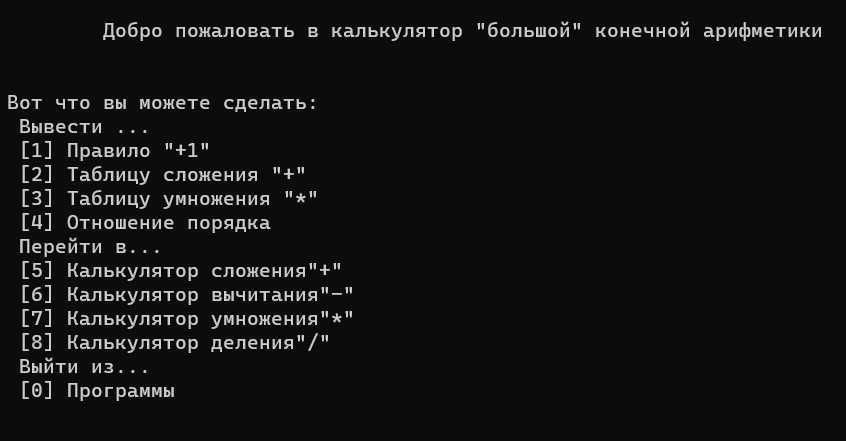
\includegraphics[width=0.8\textwidth]{3}
				\caption{Главное меню программы}
			\end{figure}
			
			После нажатия клавиши <<1>>, либо <<2>>, либо <<3>>, либо <<4>>, на консоль выводится таблица правила <<+1>>, сложения с переносом по сложению, умножения с переносом по умножению и отношение порядка соответственно (рисунки 3-8)  
			
					\begin{figure}[h!]
				\centering
				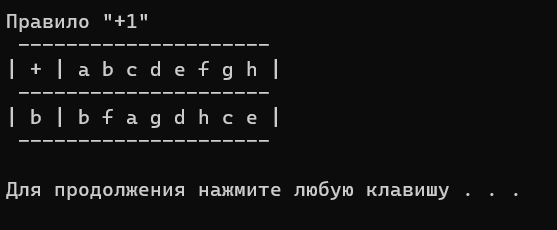
\includegraphics[width=0.7\textwidth]{4}
				\caption{Правило <<+1>>}
			\end{figure}	
			\begin{figure}[h!]
			\centering
			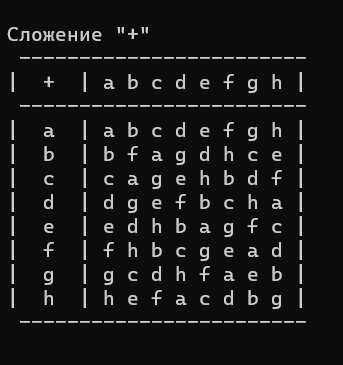
\includegraphics[width=0.35\textwidth]{5}
			\caption{Таблица сложения}
				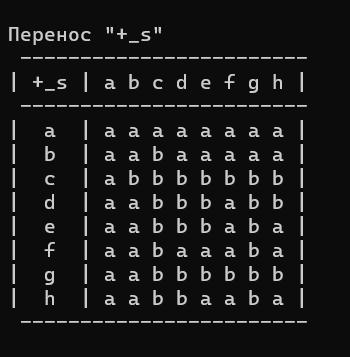
\includegraphics[width=0.35\textwidth]{6}
			\caption{Таблица переноса по сложению}
			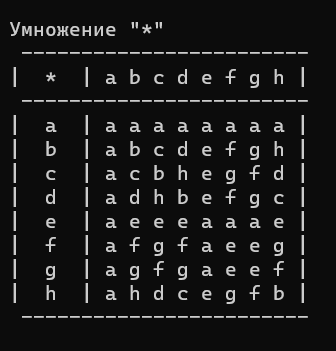
\includegraphics[width=0.35\textwidth]{7}
			\caption{Таблица умножения}
						\end{figure}
			\clearpage
				\begin{figure}[h!]
				\centering
				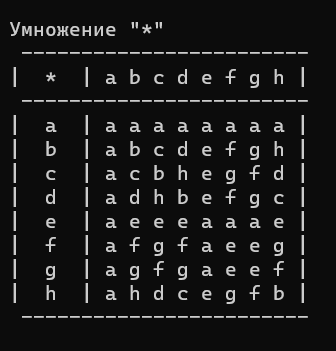
\includegraphics[width=0.35\textwidth]{8}
				\caption{Таблица переноса по умножению}
				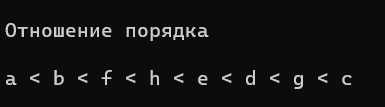
\includegraphics[width=0.5\textwidth]{13}
				\caption{Отношение порядка}
			\end{figure}
			
				После нажатия клавиши <<5>>, либо <<6>>, либо <<7>>, либо <<8>>, переход в калькулятор сложения, вычитания, умножения или деления соответвственно, затем программа запрашивает числа, после корректного ввода выводится ответ. Примеры ввода и вычисления в 4 калькулятторах изображены на рисунках 9-13.
			\begin{figure}[h!]
				\centering
				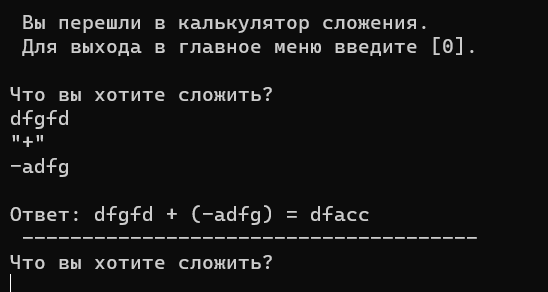
\includegraphics[width=0.5\textwidth]{9}
				\caption{Калькулятор сложения}
					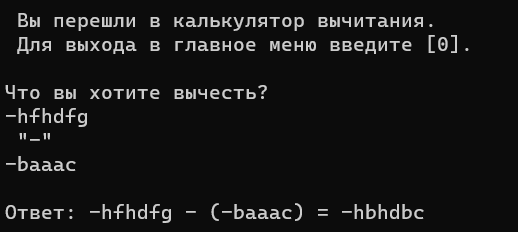
\includegraphics[width=0.5\textwidth]{10}
				\caption{Калькулятор вычитания}
			\end{figure}	
			\newpage
			\begin{figure}[h!]
			\centering
			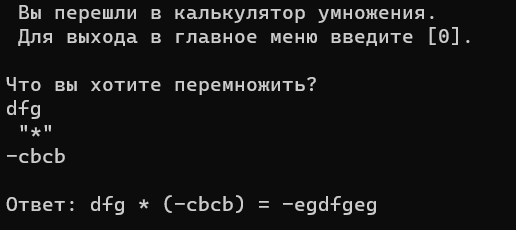
\includegraphics[width=0.5\textwidth]{11}
			\caption{Калькулятор умножения}
				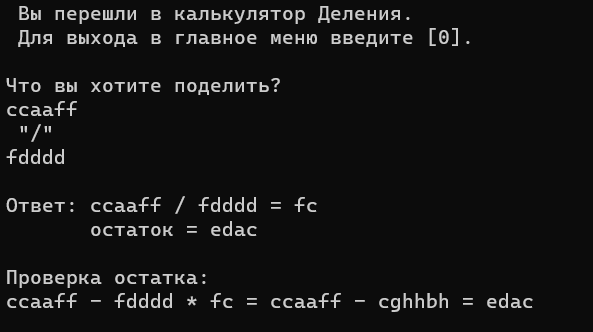
\includegraphics[width=0.5\textwidth]{12}
			\caption{Калькулятор деления}
		\end{figure}	
		
		\newpage
		\section* {Заключение}
		
		
	
		\addcontentsline{toc}{section}{Заключение}
		


	
	В результате выаолнения курсовой работы был реализован калькулятор для выполнения четырех арифметических операций $(+, -, *, \div)$ с «большими» конечными числами $<M_{8}^{8} ;+, *>$Он основан на «малой» конечной арифметике $<M_{8};+, *>$, где действует правило « +1» и выполняются обычные свойства арифметических операций, а именно коммутативности $(+,*)$, ассоциативности $(+, *)$, дистрибутивности $*$ относительно $+$, определены аддитивная единица «а» и мультипликативная единица «b». Кроме того, программа имеет защиту от неправильного ввода данных пользователем.
	
	Одним из преимуществ разработанной программы является то, что с помощью объектно-ориентированного подхода класс Ar можно расширить битовыми операциями, такими как <<И>>, <<ИЛИ>>, <<исключающее ИЛИ>>. Можно также использовать этот класс с любыми другими классами. Помимо этого, преимущество программы состоит в том, мало повторяется код, реализованы функции которые вызываются в программе в нескольких местах или являются общими для некоторых действий, тем самым не повторяя уже написанный код гдето в других местах. Например метод проверки пользовательского ввода или заполнение таблицы умнижения или деления. Вместо того чтобы написать две такие функции с практически идеальным фрагментом кода, используется одна функция, в которой меняются небольшие различия действий, взависимости от параметра
	
	Одним из недостатков является то, что пришлось использовать оптимизацию деления вручную, без нее уже для шести разрядных чисел решение находилось очень долго. Поэтому если увеличивать разрядность чисел, придется самим прописывать оптимизацию, так как при увеличении разрядностей, деление будет достаточно долго считает.
	
	
	В данной программе можно реализовть эффективную функцию деления, а также реализовать функции поиска НОД и НОК.
	
		Лабораторная реализована на языке С++, в среде разработки Visual Studio 2022.
	

		\newpage
		\section* {Источники}
		\addcontentsline{toc}{section}{Источники}
		\begin{quote}
			1. Дискретная математика для программистов. 3-е издание. Новиков Ф.А.
			СПБ:.Питер,2009.
			2. Секция «Телематика». -\href{https://tema.spbstu.ru/dismath/}{https://tema.spbstu.ru/dismath/} 
			
			3. Полубенцева М.И. С/C++. Процедурное программирование. БХВ-Петербург, 2008. 
		\end{quote}
		
	\end{document}
	
	